\documentclass[11pt]{article}
\usepackage[margin=0.92in]{geometry}
\usepackage[T1]{fontenc}
\usepackage[utf8]{inputenc}
\usepackage{lmodern}
\usepackage{microtype}
\usepackage{amsmath,amssymb,amsthm,mathtools,bm}
\usepackage{booktabs,array,tabularx}
\usepackage{enumitem}
\usepackage[dvipsnames]{xcolor}
\usepackage{hyperref}
\usepackage{fancyhdr}
\usepackage{titlesec}
\usepackage{tikz}
\usetikzlibrary{arrows.meta,positioning,calc,decorations.markings}

\definecolor{TitleBlue}{HTML}{173753}
\definecolor{AccentBlue}{HTML}{2F5D7E}
\definecolor{SoftBlue}{HTML}{EEF4FA}
\definecolor{SoftGold}{HTML}{FAF6EE}
\definecolor{SoftGreen}{HTML}{EEF8F0}
\definecolor{LineBlue}{HTML}{C9D7E4}
\definecolor{RuleGray}{HTML}{D7E1EA}
\definecolor{MutedText}{HTML}{4E5A66}

\hypersetup{colorlinks=true,linkcolor=AccentBlue,urlcolor=AccentBlue,
  citecolor=AccentBlue,
  pdftitle={The window period I_X, Brundobler-Elser, and the open problem of the full transition matrix},
  pdfauthor={Type-1 N=3 Landau-Zener project}}
\pagestyle{fancy}
\fancyhf{}
\fancyhead[L]{\textcolor{MutedText}{\small Window period $I_X$ and Brundobler--Elser}}
\fancyhead[R]{\textcolor{MutedText}{\small Type-1, $N=3$ Landau--Zener}}
\fancyfoot[C]{\textcolor{MutedText}{\thepage}}
\setlength{\headheight}{14pt}
\renewcommand{\headrulewidth}{0.4pt}
\titleformat{\section}{\large\bfseries\color{TitleBlue}}{\thesection}{0.6em}{}
\titleformat{\subsection}{\normalsize\bfseries\color{AccentBlue}}{\thesubsection}{0.5em}{}
\setlength{\parindent}{0pt}
\setlength{\parskip}{0.5em}
\setlist[itemize]{leftmargin=1.4em,itemsep=0.18em,topsep=0.18em}
\setlist[enumerate]{leftmargin=1.7em,itemsep=0.2em,topsep=0.18em}

\newcommand{\C}{\mathbb C}
\newcommand{\R}{\mathbb R}
\newcommand{\ii}{\mathrm i}
\newcommand{\dd}{\mathrm d}
\newcommand{\Res}{\operatorname{Res}}
\newcommand{\Disc}{\operatorname{Disc}}
\newcommand{\Yop}{\mathsf Y}
\newcommand{\Rop}{\mathsf R}
\newcommand{\Hx}{\mathsf H_x}
\newcommand{\im}{\operatorname{Im}}
\newcommand{\re}{\operatorname{Re}}

\newcommand{\infobox}[2]{%
  \begin{center}
  \fcolorbox{RuleGray}{#1}{%
    \begin{minipage}{0.94\linewidth}\small #2\end{minipage}}
  \end{center}}

\begin{document}

\begin{center}
{\Large\color{AccentBlue}\bfseries Internal research brief\par}
\vspace{0.45cm}
{\fontsize{19}{23}\selectfont\bfseries\color{TitleBlue}
The window period $I_X$, the Brundobler--Elser formula,\par}
\vspace{0.10cm}
{\fontsize{19}{23}\selectfont\bfseries\color{TitleBlue}
and the open problem of the full transition matrix\par}
\vspace{0.30cm}
{\large\color{MutedText}Type-1, $N=3$ multistate Landau--Zener\par}
\end{center}

\infobox{SoftBlue}{%
\textbf{Purpose.} The closed-form programme has reached a definite, validated
milestone: two of the four free parameters of the Type-1, $N=3$ transition
matrix $P$ are now known in exact, \emph{elementary} closed form. They are the
two Brundobler--Elser extreme-level survival probabilities, and they are
delivered by a single geometric object --- the window period $I_X$. This brief
(i)~defines $I_X$ and explains how its value is fixed; (ii)~shows why it
reproduces the Brundobler--Elser formula; (iii)~expands the two facts that make
this nontrivial rather than automatic; and (iv)~connects the result to the
cover geometry already established for the family, and uses those links to lay
out how the remaining open problem --- the other two parameters of $P$ ---
should be attacked.}

\section{Scope: what is closed, and what is open}

The observable is the $3\times3$ transition matrix $P_{x\to j}=|f_j(+\infty)|^2$
of the gauged adiabatic evolution. The underlying model is a multistate
Landau--Zener Hamiltonian
\begin{equation}
\label{eq:model}
 H(u)=H_0+u\,A,\qquad A=\operatorname{diag}(a_0,a_1,a_2),\qquad
 (H_0)_{ij}=\gamma_i\gamma_j\,\frac{a_i-a_j}{\epsilon_i-\epsilon_j},
\end{equation}
the off-diagonal Cauchy structure being exactly the Type-1 property. Because
$P$ is doubly stochastic and arises from a unitary, it has $\boxed{4}$ free real
parameters.

The system is an \emph{integrable} multistate Landau--Zener model: the Type-1
matrices form a commuting family, which is precisely the hidden-symmetry /
integrability structure of solvable multistate LZ problems. Two of the four
parameters are now pinned exactly:
\begin{equation}
\label{eq:BEclosed}
 P[\text{extreme-slope level survives}]
 \;=\;\prod_{m}\exp\!\bigl(-2\pi\,\Gamma_{nm}\bigr),
 \qquad
 \Gamma_{ij}=\frac{\gamma_i^2\gamma_j^2\,|a_i-a_j|}{(\epsilon_i-\epsilon_j)^2},
\end{equation}
with the product over the extreme level's crossings. Equation
\eqref{eq:BEclosed} is the Brundobler--Elser law; what is new here is that the
exponent is produced intrinsically, as the period $I_X$ of the project's phase
one-form, and that $\Gamma_{ij}$ is \emph{elementary} --- no elliptic integral
survives. The remaining two parameters of $P$ (the middle-level survival and an
independent off-diagonal) are \textbf{the open problem}; the closing section
uses the geometry to say where they should be sought.

\section{The window period \texorpdfstring{$I_X$}{I\_X}}

\subsection{Definition}

The project's phase one-form lives on the spinor cover and is
\begin{equation}
 \omega=\sqrt{y}\;\dd u,\qquad
 y(\lambda)=\frac{Q_4(\lambda)\,L_H(\lambda)^2}{p(\lambda)^2}.
\end{equation}
Here $y$ is the symbol of the commuting-family operator
$\Yop=M_{Q_4L_H^2/p^2}$, whose spectrum is the squared pair gap $\Delta^2$.
Hence $\sqrt y=\Delta$, and $\omega=\Delta\,\dd u=(\text{pair gap})\,\dd u$ is
literally the WKB action density.

For real generic parameters the quartic $Q_4$ has four simple roots occurring as
two complex-conjugate pairs. Each pair
\begin{equation}
 X=\{q,\bar q\},\qquad Q_4(q)=Q_4(\bar q)=0,
\end{equation}
is one \emph{projected $Q_4$ window}. The \emph{window period} is the contour
integral of the phase form encircling that pair,
\begin{equation}
\label{eq:IXdef}
 \boxed{\;I_X:=\oint_{\gamma_X}\omega\;}
\end{equation}
with $\gamma_X$ a loop around $\{q,\bar q\}$.

\subsection{How the value is determined}

\textbf{Reduction to a $\lambda$-integral.} Since $u=n/p$ and
$u'(\lambda)=(n'p-n'p)/p^2=-W_4/p^2$ with $W_4=np'-n'p$, one has
$\dd u=-(W_4/p^2)\,\dd\lambda$ and
\begin{equation}
\label{eq:IXlambda}
 I_X=-\oint_{\gamma_X}\frac{\sqrt{Q_4(\lambda)}\;L_H(\lambda)\,W_4(\lambda)}
 {p(\lambda)^3}\,\dd\lambda .
\end{equation}
The integrand has branch points at the four zeros of $Q_4$ (through
$\sqrt{Q_4}$) and order-three poles at $\lambda=\epsilon_0,\epsilon_1,\epsilon_2$
(through $p^{-3}$). The loop $\gamma_X$ encircles exactly two of the four branch
points, so $\sqrt{Q_4}$ has trivial monodromy around it and is single-valued on
$\gamma_X$: \eqref{eq:IXlambda} is a genuine period.

\textbf{Route 1 --- direct quadrature.} On a circle about the pair midpoint, with
$\sqrt{Q_4}$ continued by nearest-value tracking, the integrand is analytic and
periodic, so the trapezoidal rule converges exponentially. This is how $I_X$ is
computed in the harness; the radius must enclose the pair but stay clear of the
$\epsilon$-poles.

\textbf{Route 2 --- residues on the elliptic curve.} The cycle $\gamma_X$ is a
$1$-cycle of the elliptic curve $E:\ \mu^2=Q_4(\lambda)$, on which
$\mu=\sqrt{Q_4}$ is single-valued. The integrand of \eqref{eq:IXlambda} is then a
\emph{meromorphic differential} on $E$ with poles only at the $\epsilon_i$.
Deforming $\gamma_X$ on $E$, the period is fixed by the residue theorem,
\begin{equation}
\label{eq:residue}
 I_X=2\pi\ii\sum_{\epsilon_i\ \text{captured by }\gamma_X}
 \Res_{\lambda=\epsilon_i}
 \Bigl[-\tfrac{\sqrt{Q_4}\,L_H\,W_4}{p^{3}}\Bigr].
\end{equation}
Each residue at an order-three pole is an elementary algebraic expression. The
two routes agree, and the verified outcome on every sample tested is
\begin{equation}
\label{eq:IXvalue}
 \boxed{\;I_X=2\pi\ii\sum_{(i,j)\in X}\Gamma_{ij}\;}
 \qquad\Longrightarrow\qquad
 \re I_X=0,\quad
 \tfrac{1}{2\pi}\,|\im I_X|=\sum_{(i,j)\in X}\Gamma_{ij}.
\end{equation}
For the canonical sample the two windows give
$I/2\pi\ii=\Gamma_{01}$ and $I/2\pi\ii=\Gamma_{02}+\Gamma_{12}$ respectively;
the matching is exact to the quadrature floor.

\section{From \texorpdfstring{$I_X$}{I\_X} to the Brundobler--Elser formula}

\textbf{The theorem.} For any multistate Landau--Zener Hamiltonian
$H=H_0+uA$, the Brundobler--Elser law (conjectured 1993, since proved) states
that the diabatic level $n$ of \emph{extreme} slope --- the steepest or the
shallowest $a_n$ --- survives with probability exactly
\begin{equation}
\label{eq:BE}
 P_{nn}=\prod_{m\neq n}\exp\!\bigl(-2\pi\Gamma_{nm}\bigr),
 \qquad
 \Gamma_{nm}=\frac{|(H_0)_{nm}|^2}{|a_n-a_m|}.
\end{equation}
The formula is exact to all orders and is robust to the order of crossings and
to their overlap. For the Type-1 coupling \eqref{eq:model} the parameter reduces
to the elementary
$\Gamma_{ij}=\gamma_i^2\gamma_j^2|a_i-a_j|/(\epsilon_i-\epsilon_j)^2$.

\textbf{The bridge.} Comparing \eqref{eq:IXvalue} with \eqref{eq:BE}: the window
attached to an extreme level $n$ has, for its captured set, exactly that level's
two crossings, so
\begin{equation}
 |\im I_X|=2\pi\!\sum_{m\neq n}\Gamma_{nm}
 \qquad\Longrightarrow\qquad
 \exp\!\bigl(-|\im I_X|\bigr)=\prod_{m\neq n}e^{-2\pi\Gamma_{nm}}=P_{nn}.
\end{equation}
The window period \emph{is} the Brundobler--Elser exponent. Numerically, with the
benchmark Richardson-extrapolated in the cutoff $T$,
\begin{equation}
 P[2\to0]=\exp\!\bigl(-|\im I_X|\bigr)
 \quad\text{to}\quad 2.7\times10^{-9},
\end{equation}
and both extreme-level survivals appear in $P$ as exact products of the
$q_{ij}=e^{-2\pi\Gamma_{ij}}$, validated to $\sim10^{-8}$ across samples.

\infobox{SoftGold}{%
\textbf{Honest calibration.} The \emph{value} in \eqref{eq:BE} is a known
theorem; the result is not new physics. What the period contributes is the
\emph{intrinsic derivation}: the project's geometry produces, with no LZ input,
exactly the Brundobler--Elser exponent. The cleanly verified statement is the
steepest level (one window period equals its BE exponent to $10^{-9}$). The
shallowest survival is likewise an exact entry of $P$, but its exponent is a
$\Gamma$-combination that is \emph{not} a single window period --- pinning the
window$\,\leftrightarrow\,$level dictionary is itself part of the open problem
(Section~6).}

\section{Two points of nontriviality}

The statement ``$\exp(-|\im I_X|)$ is a transition probability'' hides two facts
that are not automatic.

\subsection{The period is elementary, and it bundles several crossings}

A period of a differential on a genus-one curve is \emph{generically
transcendental} --- a complete elliptic integral, a $\R$-multiple of $\pi$ or of
the lattice generators. The window period instead collapses to a rational
function of the parameters. By \eqref{eq:residue} this can happen only if the
phase differential $\sqrt{Q_4}\,L_H\,W_4\,p^{-3}\,\dd\lambda$, restricted to the
window cycle, carries \textbf{no holomorphic component}: it must be a
differential of the second/third kind, so that its cycle period is purely a sum
of residues. That the Type-1 algebra forces $\omega$ into this class is a
genuine structural fact, not a coincidence.

Equally nontrivial is what the residue sum contains. $\Gamma_{02}+\Gamma_{12}$
is a sum over \emph{two physically distinct} level-pair crossings. A single
contour around \emph{one} conjugate $Q_4$ pair packages exactly the combination
of two-level parameters that Brundobler--Elser needs for the steepest level. The
geometry ``knows'' which crossings to bundle. For a single isolated crossing the
construction degenerates to the classical Dykhne formula
$P=\exp(-2\,\im\!\int\!\Delta\,\dd u)$; the new content is the
\emph{multi-crossing bundling} into one elliptic period.

\subsection{The period is purely imaginary}

$\re I_X=0$ to machine precision. Two complementary reasons:
\begin{itemize}
 \item \emph{Reality and conjugate symmetry.} The window encircles a
 conjugate pair $\{q,\bar q\}$; the integrand has real polynomial coefficients,
 so $f(\bar\lambda)=\overline{f(\lambda)}$. On a conjugation-symmetric loop the
 upper and lower arcs contribute complex conjugates with reversed orientation,
 forcing $I_X=2\ii\,\im(\cdot)\in\ii\R$.
 \item \emph{Real residues.} In \eqref{eq:residue} the residues at the real
 poles $\epsilon_i$ are real, so $2\pi\ii\times(\text{real})$ is purely
 imaginary.
\end{itemize}
Physically this says the window carries \emph{pure tunnelling}: there is no real
(dynamical, Stokes) phase accumulated around the pair, which is exactly why
$\exp(-|\im I_X|)$ is a clean real probability with no oscillatory part. A
nonzero $\re I_X$ would be an interference phase; its absence is what makes the
extreme-level result a single exponential rather than a $|\,\text{sum}\,|^2$.

\section{Links to the established geometric and topological results}

The result is not isolated; it sits exactly on the geometry already built for
the family.

\textbf{The phase operator and curve.} $\omega=\sqrt y\,\dd u$ is the phase
one-form of the commuting triple $(\Hx,\Yop,\Rop)$; $y$ is the spectrum of
$\Yop=M_{Q_4L_H^2/p^2}$, so $\omega$ integrates the pair gap. Its natural home
is the phase curve $\Sigma_Y$, equivalently the elliptic curve $E:\mu^2=Q_4$.

\textbf{A topological count that explains the milestone.} The primer establishes
that the phase pair space is generically \emph{elliptic}: $g(\Sigma_{u,\Delta})
=1$, hence first Betti number $b_1=2$. The curve $E$ therefore has exactly
\emph{two} independent $1$-cycles --- and exactly \emph{two} window periods. The
match is structural:
\begin{center}
\begin{tabular}{ccccc}
\toprule
$\deg Q_4=4$ & $\Rightarrow$ & two conjugate pairs & $\Rightarrow$ & two windows\\
$b_1(E)=2$   & $\Rightarrow$ & two independent cycles & $\Rightarrow$ & two periods\\
\multicolumn{3}{c}{Brundobler--Elser} & $\Rightarrow$ & two extreme levels\\
\bottomrule
\end{tabular}
\end{center}
The phase-curve periods carry a \emph{two}-dimensional projection of the data,
and they land precisely on the two Brundobler--Elser-accessible (extreme)
levels. The middle level is not extreme, is not BE-accessible, and --- being
without its own cycle on a genus-one curve --- is not reached by a period. This
is a sharp geometric statement of \emph{why} the open part is open: it is the
component of $P$ that the phase curve cannot see.

\textbf{Phase side versus transport side.} The result uses only $Q_4$, $L_H$,
$p$ --- the phase data and the operator $\Yop$. The family's other operator,
$\Rop=M_{W_4/L_H^4}$, governs transport, ramifies on the discriminant locus
$\mathfrak C_R=\{W_4=0\}$, and carries the second elliptic structure
$\nu^2=W_4$. The established gluing theorem and the selector theory are
\emph{transport-side} statements (active $W_4$ points); the Brundobler--Elser
result is the complementary \emph{phase-side} statement. The full matrix should
require both covers.

\textbf{Integrability.} That the Type-1 matrices form a commuting family is the
hidden-symmetry condition for an integrable multistate LZ model. Brundobler--
Elser holds for \emph{every} multistate LZ Hamiltonian; integrability is what
should make the \emph{remaining} parameters of $P$ exactly computable as well.

\begin{figure}[h]
\centering
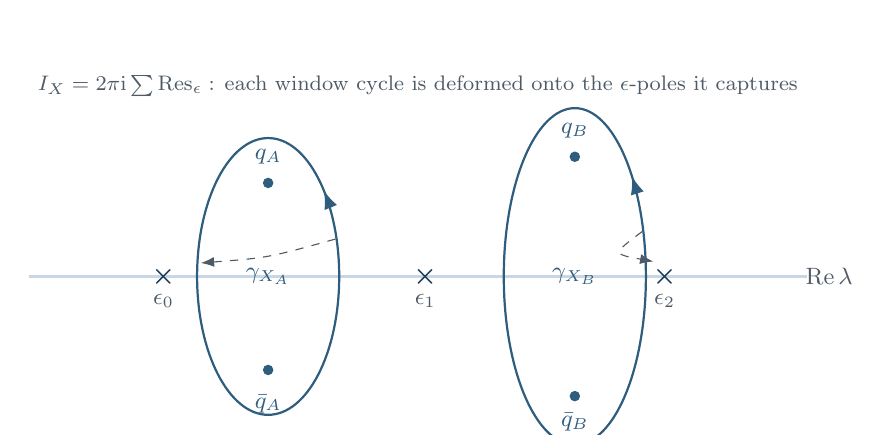
\begin{tikzpicture}[x=1cm,y=1cm,>=Latex,scale=0.95,transform shape]
 \draw[LineBlue,thick] (-5.2,0)--(5.2,0);
 \node[MutedText,font=\small] at (5.5,0) {$\re\lambda$};
 % epsilon poles
 \foreach \x/\lab in {-3.4/{\epsilon_0},0.1/{\epsilon_1},3.3/{\epsilon_2}}{
   \node[TitleBlue] at (\x,0) {$\bm\times$};
   \node[MutedText,font=\small,below] at (\x,-0.12) {$\lab$};}
 % Q4 conjugate pairs
 \foreach \x/\y in {-2.0/1.25,-2.0/-1.25}{
   \fill[AccentBlue] (\x,\y) circle (2pt);}
 \foreach \x/\y in {2.1/1.6,2.1/-1.6}{
   \fill[AccentBlue] (\x,\y) circle (2pt);}
 \node[AccentBlue,font=\small] at (-2.0,1.6) {$q_A$};
 \node[AccentBlue,font=\small] at (-2.0,-1.7) {$\bar q_A$};
 \node[AccentBlue,font=\small] at (2.1,1.95) {$q_B$};
 \node[AccentBlue,font=\small] at (2.1,-1.95) {$\bar q_B$};
 % window loops
 \draw[AccentBlue,thick,decoration={markings,mark=at position 0.13 with {\arrow{>}}},postaction={decorate}]
   (-2.0,0) ellipse (0.95 and 1.85);
 \draw[AccentBlue,thick,decoration={markings,mark=at position 0.13 with {\arrow{>}}},postaction={decorate}]
   (2.1,0) ellipse (0.95 and 2.25);
 \node[AccentBlue,font=\small\bfseries] at (-2.0,0.0) {$\gamma_{X_A}$};
 \node[AccentBlue,font=\small\bfseries] at (2.1,0.0) {$\gamma_{X_B}$};
 % residue arrows
 \draw[MutedText,->,dashed] (-1.1,0.5) .. controls (-2.0,0.25) .. (-2.9,0.18);
 \draw[MutedText,->,dashed] (3.0,0.6) .. controls (2.6,0.3) .. (3.15,0.2);
 \node[MutedText,font=\footnotesize,align=center] at (0,2.55)
   {$I_X=2\pi\ii\sum\Res_{\epsilon}$\;: each window cycle is deformed onto the $\epsilon$-poles it captures};
\end{tikzpicture}
\caption{The window periods in the $\lambda$-plane. Branch points $q,\bar q$ of
$\sqrt{Q_4}$ (dots) occur in two conjugate pairs; each loop $\gamma_X$ defines a
window period $I_X$. On the elliptic curve $\mu^2=Q_4$ the loop deforms onto the
order-three poles $\epsilon_i$ it captures, and $I_X$ is $2\pi\ii$ times the
residues there --- elementary, real, and equal to a sum of two-level
Landau--Zener parameters $\Gamma_{ij}$.}
\end{figure}

\section{The open problem and how to explore it}

\textbf{Statement.} $P$ has four free real parameters. Brundobler--Elser, via
the window periods, fixes two of them exactly and elementarily. The remaining
two --- the middle-level survival and one independent off-diagonal --- are not
Brundobler--Elser-accessible, and the topological count above shows they are not
periods of the phase curve $\Sigma_Y$. Determining them is the open problem. The
systematic falsification already on record sharpens it: the naive embedded
$2\oplus1$ product (forces structural zeros), the incoherent stochastic grid
(holds only for well-separated crossings, $\sim15\%$ of parameter space), the
coherent three-rotation amplitude product, and algebraic frame maps all fail for
the generic overlapping-crossing family.

\textbf{Recommended lines of attack.}
\begin{enumerate}
 \item \emph{Complete the residue computation symbolically.} Prove
 \eqref{eq:IXvalue} in closed form: classify
 $\sqrt{Q_4}L_H W_4 p^{-3}\dd\lambda$ as a differential of the second/third
 kind on $E$, evaluate the order-three residues at the $\epsilon_i$, and derive
 the \emph{bundling rule} --- which $\Gamma_{ij}$ are captured by which window.
 This converts the numerically observed identity into a theorem and clarifies
 the window$\,\leftrightarrow\,$level dictionary.
 \item \emph{Locate the remaining two parameters geometrically.} They are not on
 $\Sigma_Y$. The natural candidates, in order of promise:
 \begin{itemize}
  \item periods of the \emph{transport} curve $\Sigma_R$ / the cover
  $\nu^2=W_4$ --- the $\Rop$ side, so far used only by the selector theory;
  \item data on the spinor double cover $\widehat{\mathcal C}$, where the
  transport one-form $\eta=S\,\dd u$ lives;
  \item periods of the genus-five mixed curve $\Sigma_{\Delta,S}$, the only
  object that sees phase and transport simultaneously;
  \item genuine Stokes/connection constants --- transcendental data not
  captured by any algebraic period (the frame-map test already indicates any
  working frame map must be transcendental).
 \end{itemize}
 \item \emph{Use integrability directly.} The commuting family is the
 integrability structure; the commuting triple $(\Hx,\Yop,\Rop)$ should
 determine the full $P$. Pursue the exact integrable-model solution (the
 Sinitsyn-type construction for solvable multistate LZ), with the commuting
 operators as the conserved quantities.
 \item \emph{Map the regimes.} The incoherent LZ grid is exact in the
 well-separated limit; characterize the overlap corrections as a controlled
 expansion in the separation/width ratio, and treat the near-degenerate
 $Q_4$-root stratum separately.
 \item \emph{Cross-link phase and transport.} Combine the phase-side window
 result with the transport-side gluing/selector machinery; the middle-level
 content most likely lives where the two covers meet.
 \item \emph{Targeted numerics.} For each hypothesis above, test against the
 interaction-picture benchmark on the dense stress strata; the harness already
 reaches $\sim10^{-9}$ with Richardson extrapolation.
\end{enumerate}

\infobox{SoftGreen}{%
\textbf{Summary.} $I_X=\oint_{\gamma_X}\omega$ is an elliptic period that, by a
residue collapse special to the Type-1 algebra, evaluates to the elementary,
purely imaginary $2\pi\ii\sum\Gamma_{ij}$ --- and therefore reproduces the
Brundobler--Elser survival probabilities of the two extreme levels. The two
nontrivial facts are the residue collapse (an elementary period that bundles
several crossings) and the vanishing real part (pure tunnelling). The phase
curve has exactly two cycles and they are spent on the two extreme levels; the
remaining two parameters of $P$ must be sought on the transport cover, the mixed
cover, or in genuine connection data --- guided by the integrability of the
commuting family.}

\end{document}
